\section{Modello Analitico}
In questa sezione viene mostrata la metodologia utilizzata per la stima
statistiche.  Nel modello analitico le statistiche si basano sui valori medi
delle variabili aleatorie $S$, $N$ e $X$, corrispondenti rispettivamente al
tempo di risposta, popolazione e throughput.

Per il calcolo delle metriche locali e globali, è stato inoltre necessario
ottenere la distribuzione stazionaria dello stato del cloudlet, in modo tale da
poter stabilire lo stato di tutto il sistema in condizioni di stazionarietà, e a
tale scopo, si è modellato il cloudlet come una catena di markov.
%
\subsection{Calcolo della distribuzione stazionaria}
Il generico stato della catena di markov è rappresentato da una coppia di interi
($n_1, n_2$) che indicano la quantità di job della relativa classe presenti nel
cloudlet.\\
La frequenza di transizione da uno stato all'altro è regolata dai tassi di
arrivo $\lambda_1$ e $\lambda_2$ e di completamento $\mu_1^{clet}$ e
$\mu_2^{clet}$ che verranno indicati semplicemente con $\mu_1$ e $\mu_2$, poiché
la catena di markov è riferita soltanto al cloudlet.

La catena rispetta i vincoli imposti relativi alla somma delle variabili $n_1$ e
$n_2$, gli stati risultanti sono mostrati in figura~\ref{ctmc}: le freccie
tratteggiate indicano il fatto che i job, al loro arrivo, vengono direttamente
inoltrati al server remoto, mentre nel caso in cui arrivi un job di classe $1$
nello stato ($n_1, n_2$) tale che $n_1+n_2=S$, si passa allo stato ($n_1+1,
n_2-1$) e ciò rappresenta una migrazione di un job di classe 2.
%
\begin{figure}[!h]
\centering
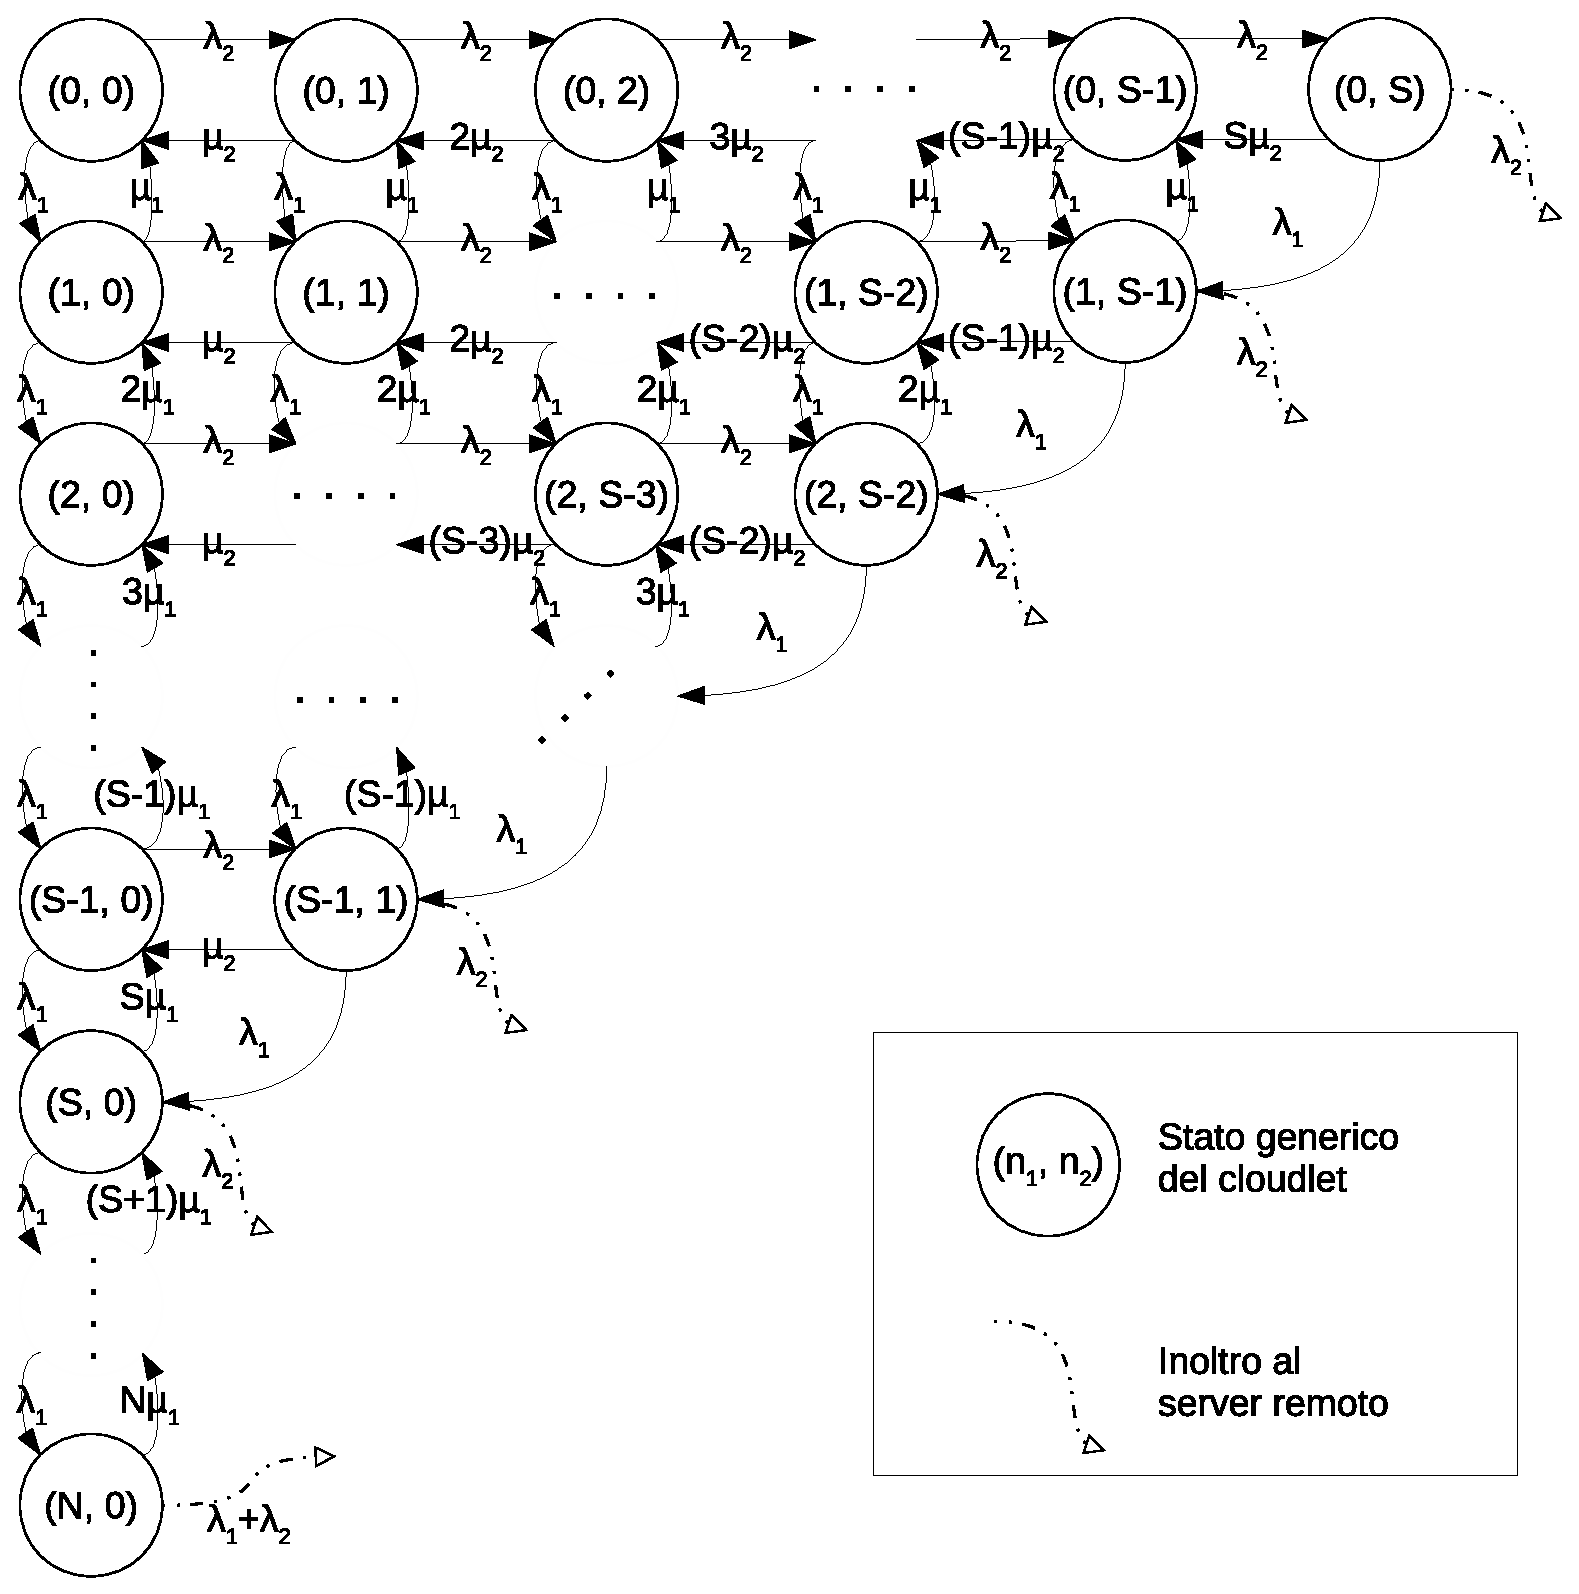
\includegraphics[width=0.7\textwidth]{figures/ctmc}
\caption{CTMC cloudlet}
\label{ctmc}
\end{figure}
%

Per il calcolo della distribuzione stazionaria si è utilizzato un programma di
calcolo basato su matrici scritto in \emph{Matlab}, al fine di risolvere il
seguente sistema di equazioni di bilancio che deriva dall'analisi della catena.

[SISTEMA DI EQUAZIONI DI BILANCIO]

In tal modo si è ricavato il vettore $x = (x_1, x_2, \ldots, x_n)$ di dimensione
$n$ pari al numero di stati della catena di markov, dove un generico $x_k$
corrisponde alla probabilità di trovarsi nello stato ($n_1, n_2$) in condizioni
di stazionarietà, e verrà indicata con il simbolo $\pi_{(n_1,n_2)}$. A questo
punto è possibile, sommando le opportune $\pi_{(n_1,n_2)}$, ricondursi alle
probabilità che si verifichino determinati eventi che consentiranno di stimare
le metriche di interesse.
%
%
\subsection{Stima delle metriche}
[INTRO]
\subsubsection{Probabilità preliminari}
Prima di tutto è conveniente sfruttare la distribuzione stazionaria per il
calcolo di alcune probabilità preliminari, utili al calcolo dei tempi di
risposta.
\begin{itemize}
\item \emph{Probabilità di Accettazione}: probabilità che il sistema si trovi in
uno stato in cui qualunque job viene accettato in esecuzione nel cloudlet
\begin{equation}
\Pi_A = \sum_{\substack{n_1,n_2:\\n_1 + n_2 < S}} \pi_{(n_1,n_2)}
\end{equation}
\item \emph{Probabilità di Soglia}: probabilità che il sistema si trovi in uno
stato in cui il valore di soglia è stato raggiunto
\begin{equation}
\Pi_S = \sum_{\substack{n_1,n_2:\\ n_1 + n_2 \geq S}} \pi_{(n_1,n_2)}
\end{equation}
\item \emph{Probabilità di Blocco}: probabilità che il sistema si trovi in uno
stato in cui qualunque job viene direttamente inoltrato al server remoto (cloud)
\begin{equation}
\Pi_B = \sum_{\substack{n_1,n_2:\\n_1 + n_2 = N}} \pi_{(n_1,n_2)}
\end{equation}
\item \emph{Probabilità di Interruzione}: probabilità che il sistema si trovi in
uno stato in cui è possibili che un job venga interrotto
\begin{equation}
\Pi_I = \sum_{\substack{n_1,n_2:\\n_1 + n_2 = N\\n_2 > 0}} \pi_{(n_1,n_2)}
\end{equation}
\item \emph{Probabilità di Interruzione a seguito di Accettazione}: probabilità
che un job accettato nel cloudlet venga interrotto, calcolata rapportando la
frequenza di interruzione di un job alla frequenza di accettazione
\begin{equation}
P_{intr} = \frac{\lambda_1 \ \Pi_I}{\lambda_2 \ \Pi_A}
\end{equation}
\end{itemize}
Da ora in poi, con il nome con ``probabilità di
interruzione'' verrà indicato il termine $P_{intr}$, poiché la probabilità
$\Pi_I$ non verrà più utilizzata nel resto dell'analisi.
%
%
\subsubsection{Tempo di risposta: Cloudlet}
Il tempo medio di risposta di un job di classe 1 per il cloudlet è banalmente il
reciproco del tasso di servizio relativo:
\begin{equation}
E[S_1^{clet}] = \frac{1}{\mu_1^{clet}}
\end{equation}
tale valore è indipendente dal paremtro $S$ ed equivale a $2.\overline2$, mentre
per quanto riguarda i job di classe 2, il tempo medio di servizio subisce una
riduzione dovuta alle interruzioni. Infatti, poiché i job che hanno un tempo
di servizio maggiore del valor medio ($1/\mu_2^{clet}$) permangono nel nodo per
più tempo, sono più soggetti alle interruzioni, quindi
non verranno inclusi nel calcolo del tempo medio ed incideranno maggiormente i
job con un tempo di servizio minore.
Si può stimare che, tale tempo di risposta medio, viene abbattuto di un fattore
$S_r$ proporzionale alla probabilità che un job venga interrotto.
\begin{eqnarray}
S_r &=& \frac{1}{\mu_2^{clet}} \ P_{intr}  \nonumber \\
E[S_2^{clet}] &=& \frac{1}{\mu_2^{clet}} - S_r
\end{eqnarray}

Tale stima è ragionevole, poiché se si ragiona al limite si ha che, in assenza di
interruzioni, il tempo di risposta assume il valore normale $1/\mu_2^{clet}$,
altrimenti, con una probabilità di interruzione pari a 1, assume giustamente il
valore nullo, poiché non ci sarebbero completamenti in tali condizioni.
\begin{eqnarray*}
P_{intr} \longrightarrow 0 \qquad & \Rightarrow \qquad & 
S_r \rightarrow 0 \ ; \qquad E[S_2^{clet}] \rightarrow
\frac{1}{\mu_2^{clet}} \ \\
P_{intr} \longrightarrow 1 \qquad & \Rightarrow \qquad & 
S_r \rightarrow \frac{1}{\mu_2^{clet}} \ ; \qquad E[S_2^{clet}] \rightarrow 0
\end{eqnarray*}

Il tempo di risposta medio globale per il cloudlet è calcolato come una media
pesata sul tipo di job di che attraversano il nodo. Nello specifico si ha che
una porzione pari a $\lambda_1/(\lambda_1+\lambda_2)$ degli arrivi totali al
cloudlet è di classe 1 e sarà in servizio per un tempo mediamente pari a
$E[S_1^{clet}]$, la restante porzione ($\lambda_2/(\lambda_1+\lambda_2)$) invece
è di classe 2 e sarà in servizio per un tempo mediamente pari a $E[S_2^{clet}]$.
Si ottiene quindi la formula seguente:
\begin{equation}
E[S_{clet}] = 
\frac{\lambda_1}{\lambda_1+\lambda_2} \ E[S_1^{clet}] +
\frac{\lambda_2}{\lambda_1+\lambda_2} \ E[S_2^{clet}] 
\end{equation}
%
\subsubsection{Tempo di risposta: Cloud}
Per quanto riguarda il cloud, i tempi di risposta specifici per classe sono
molto semplici da stimare, e sono pari al reciproco del rispettivo tasso di
servizio:
\begin{eqnarray}
E[S_1^{cloud}] &=& \frac{1}{\mu_1^{cloud}} \\
E[S_2^{cloud}] &=& \frac{1}{\mu_2^{cloud}}
\end{eqnarray}
Il tempo di risposta globale per il cloud può essere calcolato in maniera
analoga al caso del cloudlet, ad eccezione del fatto che i tassi di arrivo non
sono noti, ma possono essere calcolati facilmente perché equivalgono ai tassi di
scarto del cloudlet.

I job di classe 1 vengono scartati soltanto nel caso in cui il cloudlet si trova
nello stato $(N, 0)$, ovvero quando vi sono esattamente N job di classe 1 in
esecuzione.

I job di classe 2 vengono scartati nel caso in cui il cloudlet si trova in uno
stato in cui si è raggiunto il valore di soglia, oppure nel caso in cui avvenga
una sostituzione con uno di classe 1. In conlusione si ottiene:
\begin{eqnarray}
\lambda_1^{cloud} = \Pi_B \ \lambda_1 
\qquad\quad\qquad
\lambda_2^{cloud} = (\Pi_S + \Pi_A P_{intr}) \ \lambda_2 \nonumber\\[4pt]
E[S_{cloud}] = 
\frac{\lambda_1^{cloud}}{\lambda_1^{cloud}+\lambda_2^{cloud}} \ E[S_1^{cloud}] +
\frac{\lambda_2^{cloud}}{\lambda_1^{cloud}+\lambda_2^{cloud}} \ E[S_2^{cloud}] 
\end{eqnarray}
%
\subsubsection{Tempo di risposta: Sistema}
Un job di classe 1, al suo arrivo nel sistema, può essere soggetto a due
alternative: essere inoltrato nel cloud nel caso in cui il cloudlet sia saturo
con probabilità $\Pi_B$, oppure essere eseguito nel cloudlet con probabilità
$1-\Pi_B$.
\begin{equation}
E[S_1] = (1-\Pi_B) \ E[S_{clet}] \ + \ \Pi_B \ E[S_{cloud}]
\end{equation}

Prima di calcolare il tempo di risposta medio dei job di classe 2, è necessario
calcolare il tempo di risposta medio di un job interrotto.\\
Tale tempo è composto dalla somma di tre componenti, partendo dall'ultima: il
tempo medio di servizio nel nodo cloud pari a $E[S_{cloud}]$, il tempo medio di
setup pari a $E[S_{setup}]$ ed infine il tempo medio di esecuzione nel cloudlet
prima che il job venga interrotto.

La stima di quest'ultimo può essere effettuata similmente a quella del calcolo
del tempo di risposta dei job di classe 2 nel cloudlet. Infatti anche in questo
caso è necessario sottrarre un certa quantità al tempo che normalmente avrebbe
impiegato in esecuzione se non ci fosse stata interruzione, ovvero
$1/\mu_2^{clet}$. Sarebbe quindi ideale la relazione del tipo:
\begin{displaymath}
E[Y] = \frac{1}{\mu_2^{clet}}(1 - \beta P_{intr})
\qquad\quad\qquad 0 < \beta \leq 1
\end{displaymath}
perché si vuole che il tempo di esecuzione antecedente all'interruzione (qui
indicato per semplicità con $Y$) diminuisca all'aumentare della probabilità di
interruzione. Si noti che per $\beta = 1$ si ottiene esattamente la formula di
$E[S_2^{clet}]$, in questo caso però, non si vuole che il tempo di esecuzione
tenda a 0 se la probabilità di interruzione fosse pari a 1, perché tale
situazione non sarebbe realistica, infatti anche se ogni singolo job deve essere
interrotto non si può pensare che esso abbia un tempo di esecuzione nel cloudlet
pari a 0. Per questo motivo, $\beta$ funge da fattore di attenuazione che riduce
l'incisività della probabilità di interruzione sul calcolo.

Tramite il confronto congiunto con le varie simulazioni al variare del parametro
$S$, è stato scelto il un valore del fattore $\beta$ pari a $0.95$. Si è giunti
quindi alla formula seguente per il calcolo del tempo medio di servizio di un
job interrotto:
\begin{equation}
E[S_{intr}] = 
(1 - \beta P_{intr}) \frac{1}{\mu_2^{clet}} + E[S_{setup}] + E[S_{cloud}]
\qquad\quad \beta = 0.95
\end{equation}

Un job di classe 2 invece può avere tre diversi tempi di esecuzione in base ai
seguenti casi:
\begin{itemize}
\item[-]Il job viene inoltrato direttamente al cloud remoto perché si è
raggiunto il valore di soglia, dove viene eseguito per un tempo mediamente pari
a $E[S_2^{cloud}]$, questo avviene con probabilità $\Pi_S$;
\item[-]Il job viene accettato nel cloudlet e non viene interrotto, il suo tempo
di esecuzione è mediamente pari a $E[S_2^{clet}]$, questo accade con probabilità
$\Pi_A (1 - P_{intr})$;
\item[-]Il job viene eseguito nel cloudlet, viene interrotto ed inoltrato al
server remoto in cui viene eseguito dopo una fase di setup, questo avviene con
probabilità $\Pi_A P_{intr}$ ed il tempo di esecuzione è mediamente pari a 
$E[S_{intr}]$; 
\end{itemize}
Pertanto un job di classe 2 ha un tempo di risposta medio che deriva dalla
seguente formula:
\begin{equation}
E[S_2] \ = \
\Pi_S E[S_2^{cloud}] \ + \ \Pi_A (1-P_{intr}) E[S_2^{clet}] \ + \ 
\Pi_A P_{intr} E[S_{intr}]
\end{equation}
Il tempo di risposta globale del sistema è calcolato analogamente al caso del
cloudlet, con i tempi di servizio riferiti al sistema intero, si ha quindi:
\begin{equation}
E[S] \ = \
\frac{\lambda_1}{\lambda_1+\lambda_2}  E[S_1] \ + \
\frac{\lambda_2}{\lambda_1+\lambda_2}  E[S_2] 
\end{equation}
%
%
\subsubsection{Popolazione media: Cloudlet}
La popolazione media del cloudlet, sia per classe che globale, viene calcolata
sommando il prodotto, relativo ad ogni stato, tra il numero di job presenti in
esso per la probabilità di trovarcisi in condizioni di stazionarietà, ovvero:
\begin{eqnarray}
E[N_1^{clet}] &=& \sum_{(n_1,n_2)} n_1 \ \pi_{(n_1,n_2)} \\
E[N_2^{clet}] &=& \sum_{(n_1,n_2)} n_2 \ \pi_{(n_1,n_2)} \\
E[N_{clet}] &=& \sum_{(n_1,n_2)} (n_1+n_2) \ \pi_{(n_1,n_2)} 
\end{eqnarray}
%
\subsubsection{Popolazione media: Cloud}
Per il calcolo della popolazione media del cloud si può sfruttare il fatto che
il nodo ha risorse virtualmente infinite (utilizzazione $\rho < 1$), pertanto si
può considerare stabile ed è possibile applicare la legge di Little:
\begin{eqnarray}
E[N_j^{cloud}] &=& \lambda_j^{cloud} E[S_j^{cloud}]  \qquad\quad\qquad j=1,2 \\
E[N_{cloud}] &=& (\lambda_1^{cloud} + \lambda_2^{cloud}) E[S_{cloud}]
\end{eqnarray}
%
\subsubsection{Popolazione media: Setup}
Anche il nodo di setup può essere considerato stabile per gli stessi motivi.
Si può applicare la legge di Little con un tasso di arrivi a questo nodo pari al
tasso di interruzione dei job di classe 2.
\begin{eqnarray}
\lambda_{setup} &=& \Pi_A P_{intr} \ \lambda_2    \nonumber \\
E[N^{cloud}] &=& \lambda_{setup} \ E[S_{setup}] 
\end{eqnarray}
%
\subsubsection{Popolazione media: Sistema}
Anche il sistema si può considerare stabile, perché globalmente ha anch'esso
risorse infinite.
\begin{eqnarray}
E[N_j] &=& \lambda_j E[S_j]  \qquad\quad\qquad j=1,2 \\
E[N] &=& (\lambda_1 + \lambda_2) E[S]
\end{eqnarray}
%
\subsubsection{Throughput}
Per il calcolo del throughput si può sfruttare sempre la condizione di stabilità
del sistema e dei suoi nodi, e poi calcolare il throughput del cloudlet
sottraendo dal throughput del sistema quello del cloud, poiché le uscite dal
nodo di setup non corrispondono a quelle del sistema.
\begin{eqnarray}
X_j^{cloud} &=& \lambda_j^{cloud}   \qquad\quad\qquad\quad j=1,2 \\
X_{cloud} &=& \lambda_1^{cloud} + \lambda_2^{cloud}   \\
X^{setup} &=& \lambda_{setup}   \\
X_j &=& \lambda_j  \ \quad\qquad\quad\qquad \ \quad j=1,2 \\
X &=& \lambda \\
X_j^{clet} &=& X_j - X_j^{cloud} \\
X_{clet} &=& X - X_{cloud} \quad\qquad\quad j=1,2
\end{eqnarray}
